% Problem ID: 106
% Original file: PAS/분해_재구성.tex


\numbering 사각형 $ABCD$ 가 중심이 $O$ 인 원에 내접하고  $\overline{AC} \bot \overline{BD}$ 일 때, 
꺾은 선  $AOC$ 는 사각형 $ABCD$ 의 넓이를 이등분한다.

\begin{center}
\resizebox{5cm}{5cm}{%
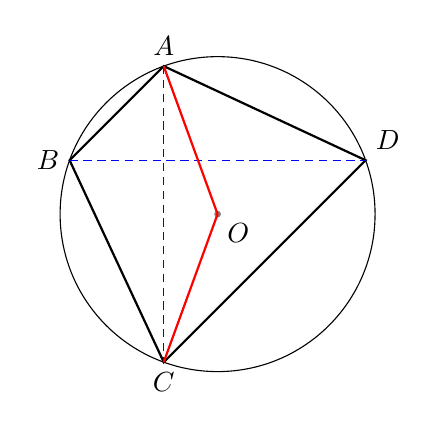
\begin{tikzpicture} 
	\draw (0,0) coordinate (O) node[below right] {$O$} circle(2);
	\draw[fill, gray] (O) circle(1pt);
	
	\draw[thick] (110:2) coordinate (A) node[above] {$ A$} 
		-- (160:2) coordinate (B) node[left] {$ B$}
		-- (-110:2) coordinate (C) node[below] {$ C$} 
		-- (20:2) coordinate (D) node[above right] {$ D$} 
		-- cycle;
		
	\draw[densely dashed, blue, thin] (A)--(C) (B)--(D);
	\draw[red, thick] (A)--(O) (O)--(C); 
\end{tikzpicture} }
\end{center}
